\documentclass[twoside,11pt]{article}

%%%%% PACKAGES %%%%%%
\usepackage{pgm2016}
\usepackage{amsmath}
\usepackage{algorithm}
\usepackage[noend]{algpseudocode}
\usepackage{subcaption}
\usepackage[utf8]{inputenc}		%NOT USED?
\usepackage[english]{babel}		%NOT USED?
\usepackage{paralist}			%NOT USED?
\usepackage[lowtilde]{url}
\usepackage{fixltx2e}

%%%%% MACROS %%%%%%
\algrenewcommand\Return{\State \algorithmicreturn{} }
\algnewcommand{\LineComment}[1]{\State \(\triangleright\) #1}
\renewcommand{\thesubfigure}{\roman{subfigure}}

%%%%% HEADING %%%%%%
% Heading arguments are {volume}{year}{pages}{submitted}{published}{author-full-names}
%\pgmheading{1}{2000}{1-48}{4/00}{10/00}{Cory J. Butz, Jhonatan S. Oliveira, André E. dos Santos, and Anders L. Madsen}


%%%%% SHORT HEADING %%%%%%
% Short headings should be running head and authors last names

%% My commands
\newcommand{\thistitle}{{Getting Started with Meteor.js}}

\ShortHeadings{\thistitle}{Oliveira}
\firstpageno{1}

\begin{document}

\title{\thistitle}

\author{\name Jhonatan S. Oliveira \email oliveira@cs.uregina.ca \\
\addr Department of Computer Science \\
University of Regina \\ 
Regina, Canada
}

\editor{CS807 - Advanced Architecture - Dr. Gerhard}

\maketitle

\begin{abstract}%   <- trailing '%' for backward compatibility of .sty file
Meteor is considered a full-stack javascript framework.
That is, it handles from the server and data modeling to the client and user interface.
Besides this all, Meteor uses only javascript as its programming language, meaning that a whole application may be build using only javascript.
Moreover, the framework incorporate reactive programming features.
Here, the flow of the data is more focused.
In Meteor, this is tracked by using events.
A general application using the framework will keep track of events and modify database and user interface accordingly.
In this paper, we also show how Meteor can be used in resource constrains computing applications to distribute computing tasks in servers and letting the client with lightweight tasks.
\end{abstract}

\begin{keywords}
Meteor, javascript, resource constrains
\end{keywords}

% Sections
\section{Introduction}
\label{sec:intro}
\section{History and Background}
\label{sec:back}

The Meteor platform was created by a company called Skybreak in 2011 \citep{skybreak}.
Later, in 2012, the company changed its name to Meteor.
The startup was incubated by YCombinator \citep{ycomb} and after receiving an investment of \$11.2 M, the platform development increased considerably.
The platform left beta in October 26th, 2015, with a version that currently provides multiplatform support.

Regarding its internal structure, Meteor is built on top of \emph{Node.js} \citep{node}.
That means that Meteor is driven by events, in order to create an asynchronous model.
This feature is implemented using callback functions: when an event happens a specific function is called to execute a portion of code.
The server-side and client-side ar both implemented using javascript.
In the client-side, templates are used to design user interfaces.
Here, a simple markup language defines the design and the events handles by the application.
Meteor has support for more than one template language, being \emph{Blaze} \citep{meteor} the official one.
In the server-side, Meteor handles data management using collections.
The oficial non-SQL database supported is MongoDB, but new ones are being incorporated in future versions \citep{fathom}.
\section{Critic}
\label{sec:new}

We start by first commenting on the proposed work itself.
SPNs are a very promising PGM.
Its feature to improve learning is of practical value, but the model was mathematically introduced with satisfactory rigour.
The model has internal characteristics which are feasible to test in practice.
These internal characteristics tells when the model will be able or not to run inference in reasonable time.
Thus, one can learn a SPN while watching for these characteristics to be controlled.
In this way, the learned model is guaranteed to do inference.

Besides that, the authors based their work on the arithmetic circuits (ACs) from \cite{Darwiche2009}.
This credit is stated right at the beginning of the paper and later one when comparing their proposed model with related works.
The relation between ACs and SPNs though could be further clarified.
It is possible to detect the similarities from the definitions, but there is a lack of clear motivation that would differentiate an AC model from a SPN.
Indeed, in \cite{Zhao2015} the authors emphasize the relation between ACs and SPNs.
In that work, it is clear that SPNs are defined in a way to be a standalone model.
It is worth mentioning that ACs are formally defined to be a compilation of a given BN.
That is, one could see an AC as an alternative way of telling the BN.
In this sense, defining a SPN as a standalone model implies in having the same expressivity of an AC with the extended feature of modelling any other possible probability distribution that fits into the internal characteristics of a SPN.
This is a very nice point to make in the paper, although it is obfuscated by technical discussion on the model itself.

A personal opinion on the proposed model would be with the lack of semantic on it.
Consider other PGMs, for instance a BN.
One can tell the relationship between variables and even infer other ones by using a BN.
On the contrary, a SPN does not have enough semantic to describe these relations neither a easy way of inferring them.
That is, learning a SPN might be beneficial but the user loses the ability of understanding the learned variables and its interactions.

Now, we comment on the paper itself.
The work is careful described.
This can be seen by the good division and flow of ideas.
The introduction is well motivated and makes an overview of the whole paper.
It also comments on related works, which gives a mor current context to the proposed work.
The Sum-Product Networks section describes the model with formal definitions and common examples.
This makes the new work more easy to follow and show its soundness.
We notice though a small lack of background information on this section.
For instance, the new model is introduced in page 2 of the paper, after a brief paragraph of definitions and contextualization.
The missing background can be of course caused by the lack of space in a conference paper, but this does not affect the work enough to stop the reader of understanding the proposed ideas.
The proofs are short and could have been more smooth, but again this can be due to the lack of space.
Section 3 makes a good comparison with relates models, which emphasize the relevance of the new work and how it overcome the other models' issues.
The following section on Learning Sum-Product networks is just a brief overview of the method, but enough to describe how one can learn a SPN from historical data.
The most impressive section is the experiment results, which shows a SPN beating famous deep architecture models in a practical application of facial completing.
This ends the paper with a very good impression.

The authors also have one section before the conclusion to talk about one possible relation between SPNs and the cortex.
They associate sum and product nodes of a SPN with two different types of cortex neurones.
This serve as a motivation for neuroscience applications that could flourish from the usage of SPNs.
Besides that, it also motivate the study of how this relationship can be beneficial for the SPNs itself.

\section{Applications}
\label{sec:app}

In order to test the abilities proposed for memcomputers, \citep{DiVentra:2012fh} did an experiment with the problem of finding the shortest path.
The problem of the shortest path is the procedure of finding a way to connect two points in a matrix via the shortest path of points between them.
It is known that this problem has complexity of logarithmic time \cite{shortestPath}.

The proposed memcomputer architecture is a square matrix made of memelements with resistive characteristic, as shown in Figure \ref{fig:square}.
Here, the architecture is a non-programable computer with memelements connected in a square format to each other.
It is worth mentioning that this memcomputer is specifically projected to solve the shortest path, that is it is not programmable for other functionalities other than that.
Also, notice that each memelement has a switch attached to it, which provides the possibility of writing and reading individually.
This is requires for initialization purposes as well as reading the result after the computation.

\begin{figure}[hbt]
    \begin{center}
    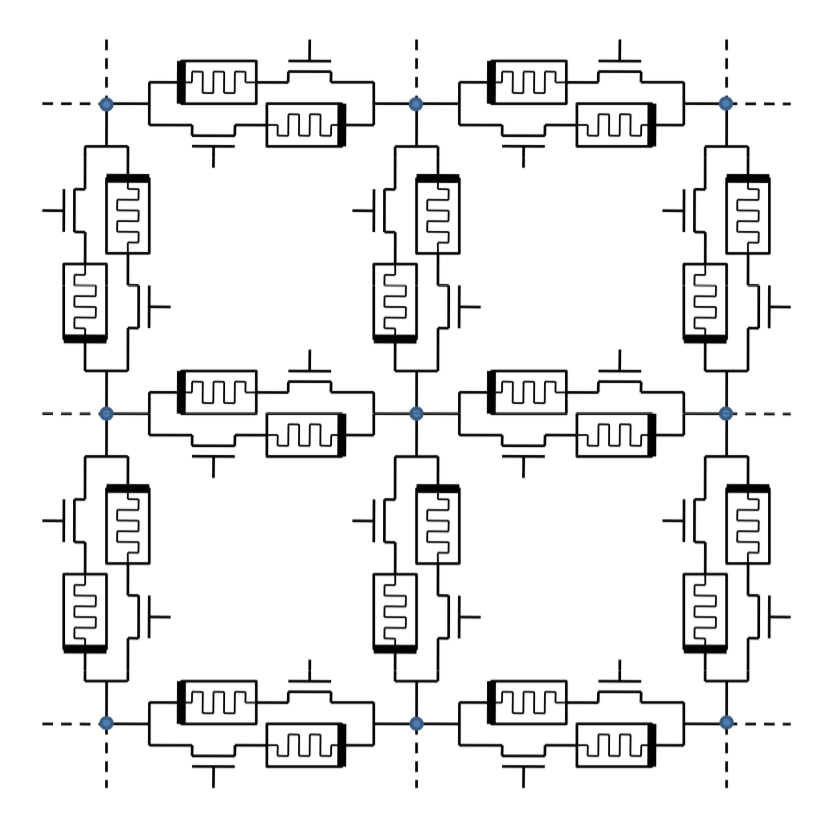
\includegraphics[width=0.5\textwidth]{figures/memcomputer.png}
    \caption{A memcomputer proposed in \citep{DiVentra:2012fh} for solving the shortest path problem.}
    \label{fig:square}
    \end{center}
\end{figure}

In this computer, we give the inputs by activating a subset of points in this grid, that is by applying a voltage in a subset of memelements.
The processing part is the collective evolution of the states of the memelements after the input is applied.
Lastly, the result of the processing step is the final state of all memelements.

The shortest path problem can be be computed using the memcomputer in Figure \ref{fig:square} by applying a constant voltage to two points the square.
These are the required input.
The memelements closer to the application of the voltage is affected by the electron current around.
Therefore, the memelement changes its resistance by lowering it down, that is the memelement become active.
The closest memelement activates itself similarly, forming a reinforcement path.
In this way, a path from the first application point to the second one is formed.
The final state that can be read from the memcomputer is a straight line of active memelements from the first point to the second one, which is the shortest path in this square.
\section{Conclusions}
\label{sec:conc}

Meteor is a simple platform for building reactive applications on the Web 2.0 paradigma.
Its event drive method offers a real time experience for the users, besides a clear division between client and server sides tasks.
Thus, Meteor can be used in resource constrain products by providing a solution when splitting workload among the more powerful server and the lightweight client.

\vskip 0.2in
\bibliography{references/references}
\end{document}
